\section{Data Analysis with De-Noising}

In this section, we compare results from the analysis of the background merged data sample with files that were de-noised prior to running through CLAS12 reconstruction software. The comparison is done for data samples with different luminosities (namely $45~nA$, $95~nA$, and $150~nA$ electron beam incident on a $5cm$ long liquid hydrogen target). The data for the raw sample and the de-noised sample is processed with the same settings of CLAS12 reconstruction software and the tracks reconstructed in each sample are analyzed.

\subsection{Luminosity dependence}

The track reconstruction efficiency is calculated according to Eqs.~(\ref{eq::eff}), (\ref{eq::eff2}) and (\ref{eq::eff3}) for positive and negative charged particles. The results are shown in Figure~\ref{lscan::conv_dn}. The track reconstruction efficiency is an integrated quantity over the particle phase space. In our studies, we used a pre-selected simulation sample of three particles in the final state, which does not necessarily have angular and momentum dependence similar to experimental data and the efficiency dependence on beam current can reflect this. In these studies, we show a relative increase in efficiency when our methods are applied to simulated data.

\begin{figure}[!h]
\begin{center}
 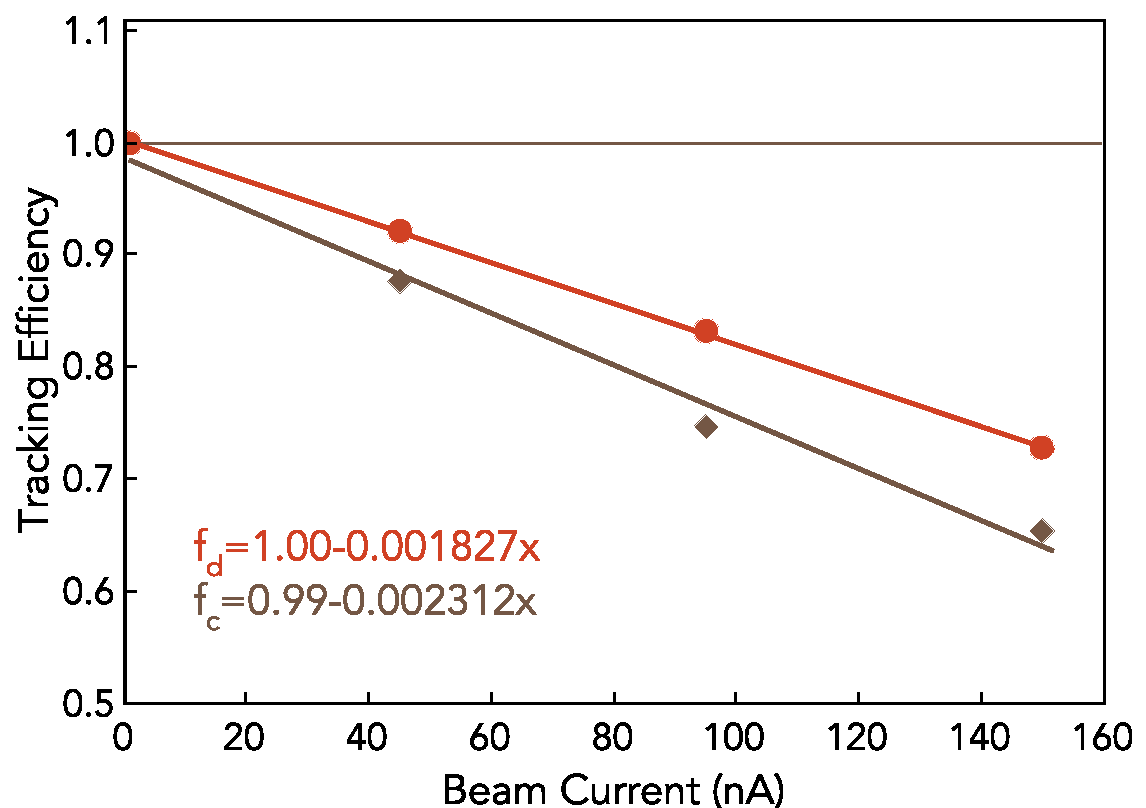
\includegraphics[width=3.1in]{images/figure_lscan_pos.pdf}
 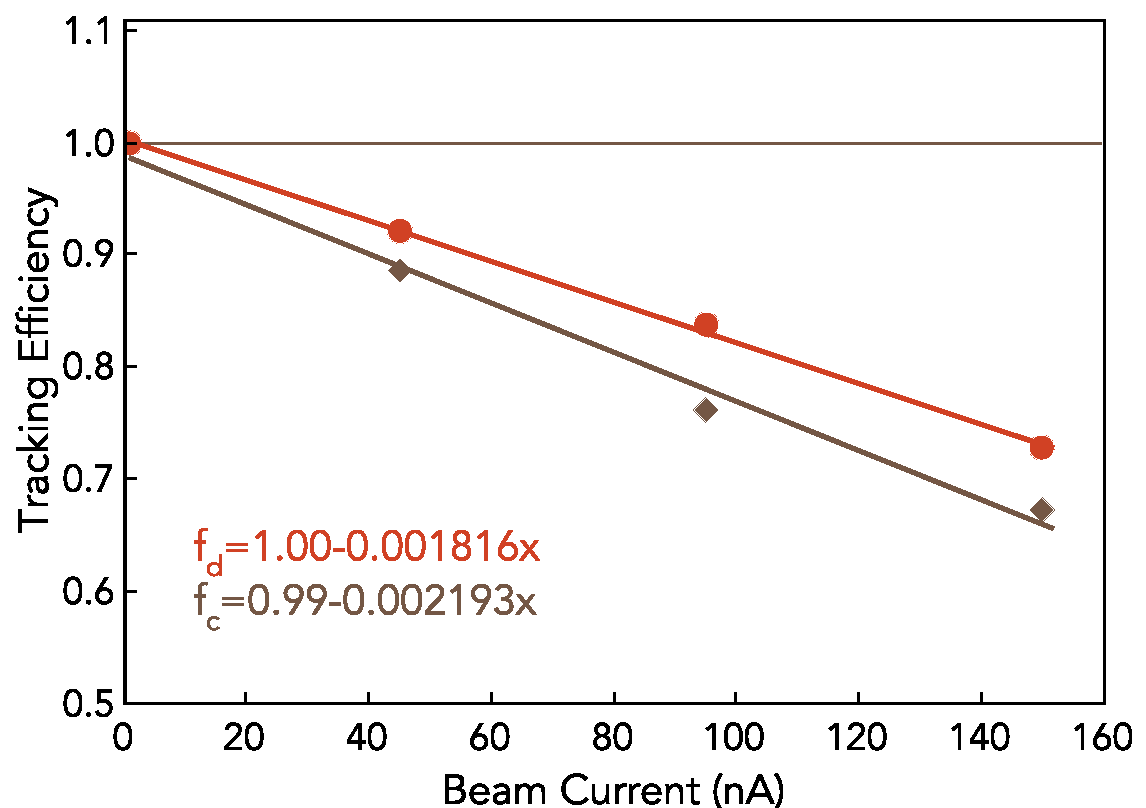
\includegraphics[width=3.1in]{images/figure_lscan_neg.pdf}
\caption {Tracking efficiency as a function of luminosity (beam current) for positively (a) and negatively (b) charged particle.  The efficiency is shown for
conventional algorithm running on background merged files (diamonds), and on files with merged background then de-noised with AI (circles).}
 \label{lscan::conv_dn}
 \end{center}
\end{figure}

As can be seen from the figure the number of reconstructed hadron-electron pairs relative to the number of reconstructed electrons is higher for the de-noised data sample compared to the raw data sample. This is due to an increased number of clusters reconstructed by the conventional clustering algorithm in the de-noised data samples. Detailed studies of cluster reconstruction efficiency are performed 
in our previously published article~\cite{Thomadakis:2022zcd}. 
The results show that the slope of the efficiency degradation as a function of the luminosity is significantly improved in the de-noised data sample. 
it is worth nothing that the track reconstruction efficiency at 75 nA with de-noised data sample track reconstruction efficiency is the same as for the 
$45~nA$ when reconstructing raw data sample (without de-noising). This implies that the experiment can run effectively at $75~nA$, collecting data 
twice faster while maintaining the same track reconstruction efficiency, which will lead to higher experimental significance in measured observables. 

\subsection{Physics Impact}

The processed data was also evaluated to extract physics observables from both data samples to discern the impact on physics for the de-noising algorithm. As mentioned before, the data selected from the Pythia simulation was for the final state $H(e,e^\prime\pi^+\pi^-p)X$ containing exactly four charged particles. From this sample the missing mass distribution of $H(e,e^\prime\pi^+\pi^-)X$ is analyzed showing a peak around proton mass where the selected reaction is inclusive $\rho$ meson production and some background (above proton mass) where other reactions  are present (with missing neutral particles).

\begin{figure}[!h]
\begin{center}
 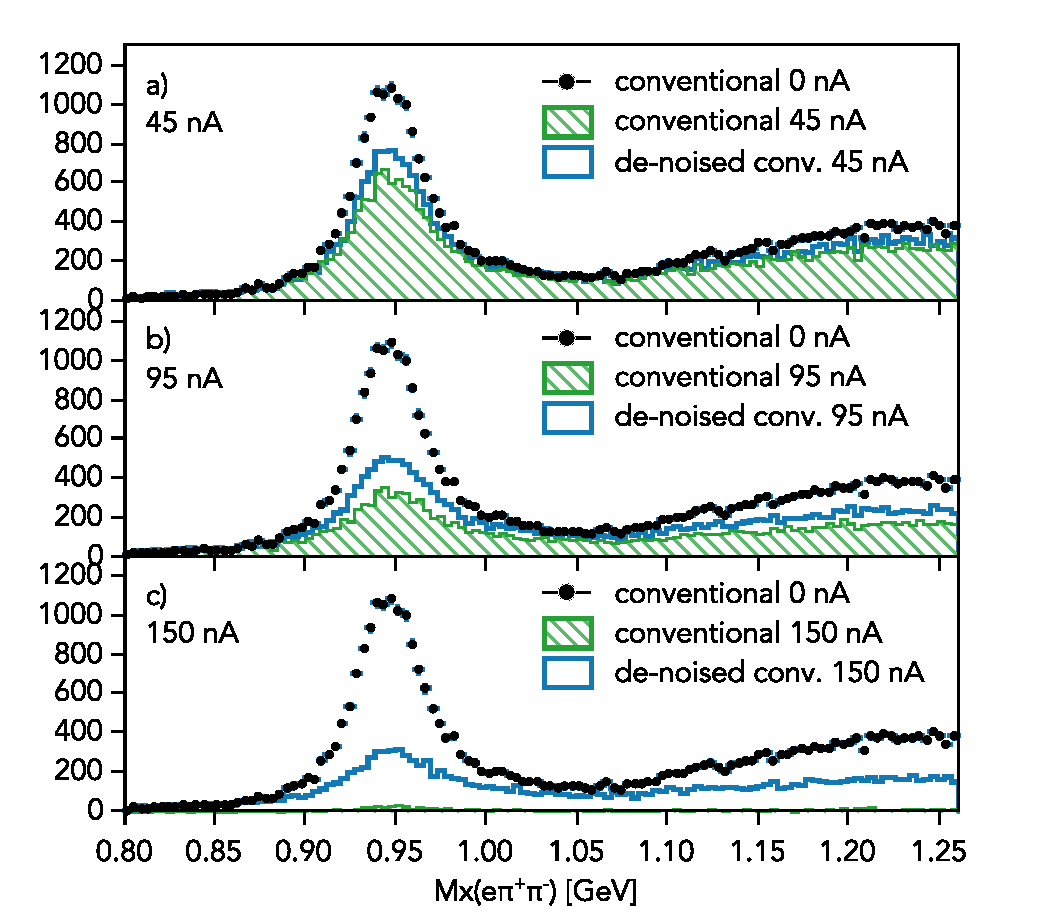
\includegraphics[height=3.1in]{images/plots_mxepipi_dn_ns.pdf}
   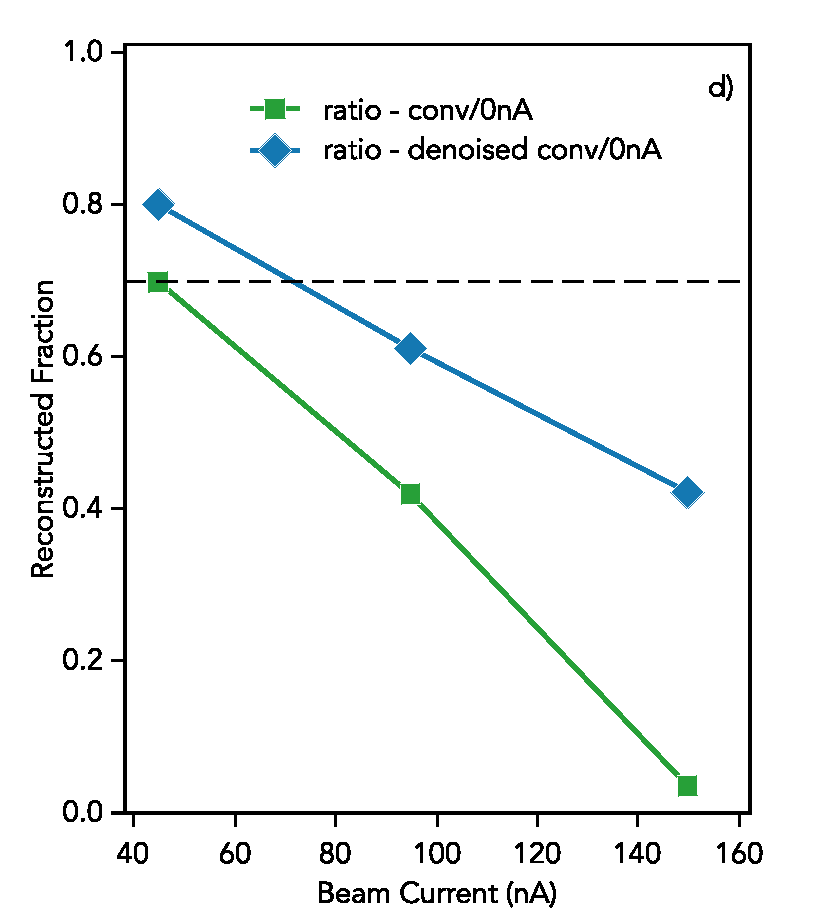
\includegraphics[height=3.1in]{images/graph_mxepipi_dn_ns.pdf}
\caption {
The de-noised data sample 
reconstructed with conventional algorithm (diamonds) for $45~nA$, $95~nA$ and $150~nA$. a), b) and c) reconstructed 
missing mass distributions for background merged data set reconstructed with conventional tracking (filled histogram) and
de-noised data sample reconstructed with conventional algorithm (solid line histogram).
d) The number of reconstructed protons from missing mass of $H(e \rightarrow e^\prime \pi^+\pi^-)X$ 
for background merged data set reconstructed with conventional tracking (squares) compared to de-noised data sample 
reconstructed with conventional algorithm (diamonds) for $45~nA$, $95~nA$ and $150~nA$.  }
 \label{physics::conv_dn}
 \end{center}
\end{figure}

In Figure~\ref{physics::conv_dn} the results of the analysis are shown, where the missing mass distribution $H(e,e^\prime\pi^+\pi^-)X$ is shown for different beam currents, in panels a), b) and c) the histograms show relative reconstructed distributions. The graph with points shows the missing mass reconstructed by the conventional tracking algorithm before any background is $0~nA$ for reference. The filled histogram shows the missing mass distribution reconstructed from background merged data with the conventional algorithm. The solid line histogram is the missing mass distribution reconstructed by a conventional algorithm after the background merged file is processed with a de-noising neural network to remove noise hits.
The summary of the number of protons in the missing mass distribution relative to the original (no background merged) distribution is presented in Figure~\ref{physics::conv_dn} d). It can be seen from the figure that the conventional algorithm reconstructs more tracks after de-noising the data. The number of reconstructed proton final states at $75nA$ from de-noised data is equal to the number of reconstructed final states at $45nA$ when using conventional track reconstruction algorithms.  Conducting experiments with higher incident beam current allows accumulating the necessary statistics for the proposed experiments in significantly less time, leading to huge savings in accelerator operations.

%\begin{figure}[!ht]
%\begin{center}
 %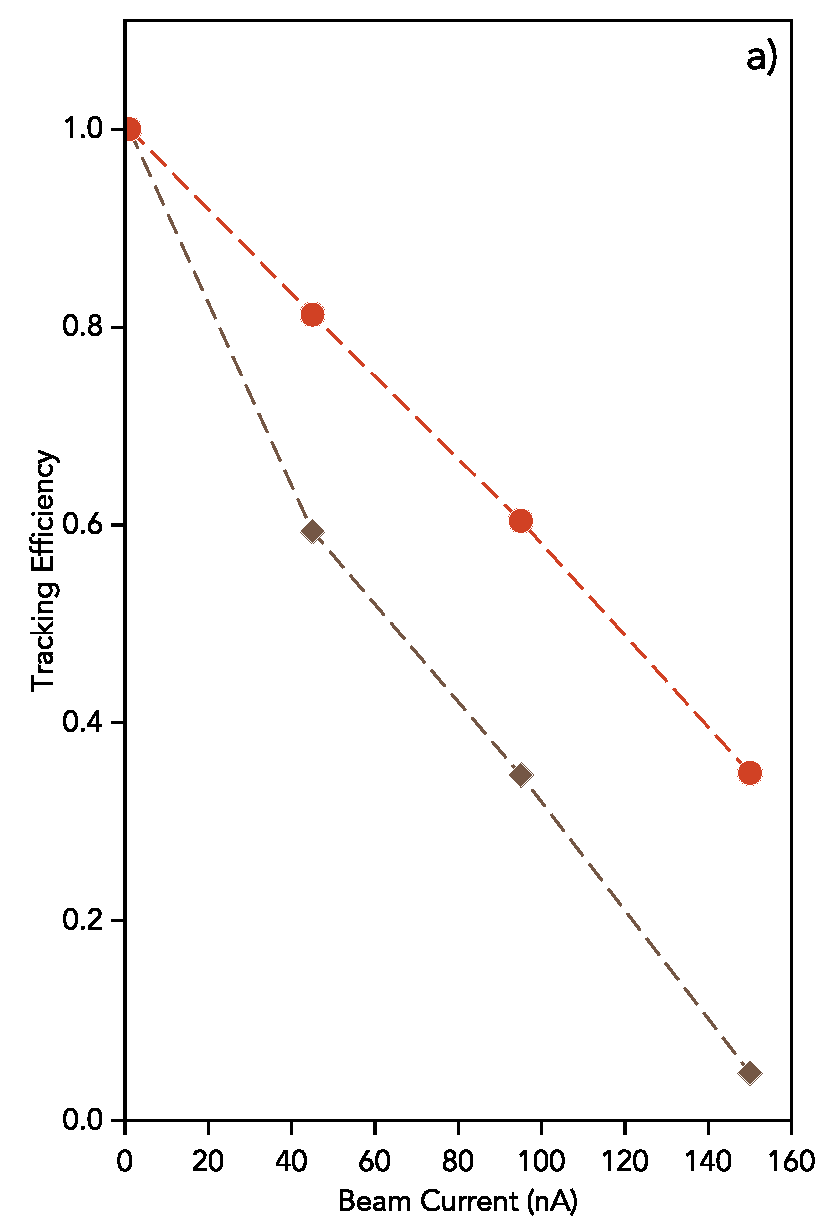
\includegraphics[width=3.1in]{images/figure_phys_scan.pdf}
 %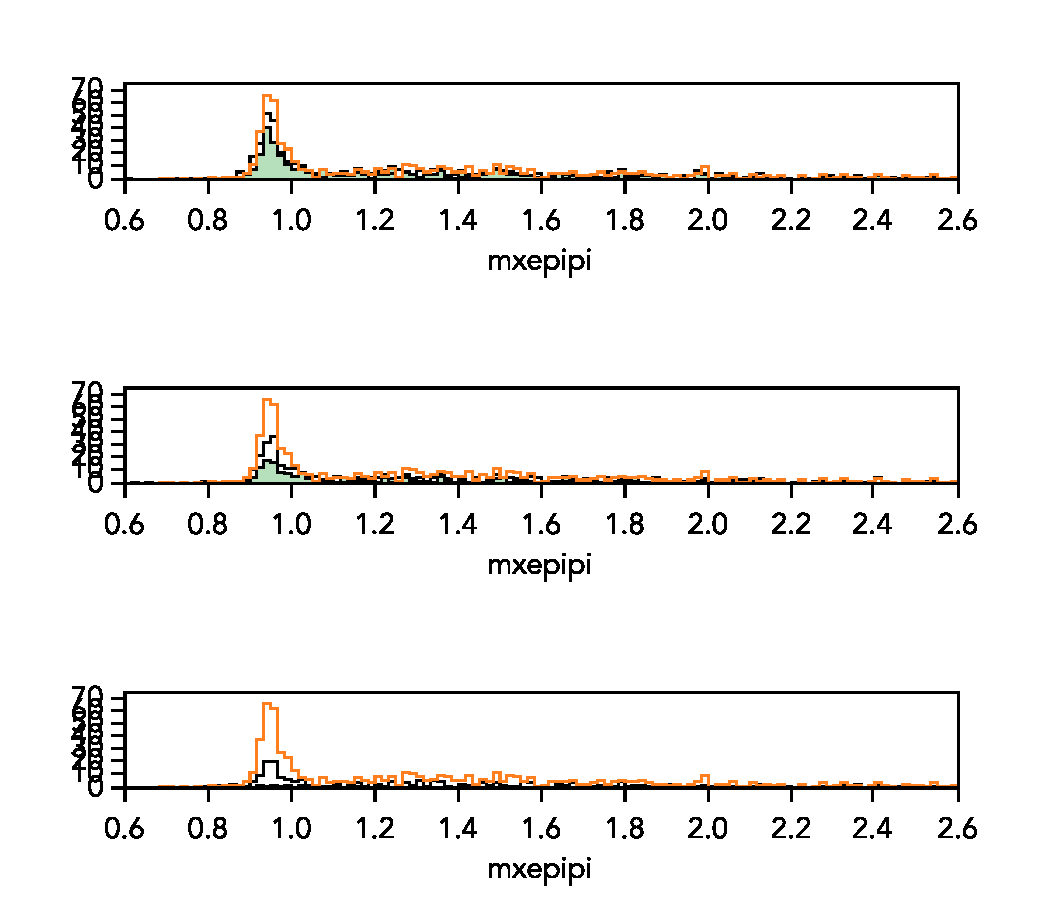
\includegraphics[width=2.5in]{images/figure_phys_conv_compare.pdf}
%\caption {Number of reconstructed protons from missing mass 
%of $H(e e^\prime \pi^+\pi^-)$ for background merged files for 
%$5~nA$, $45~nA$, $95~nA$ and $150~nA$ respectively.}
 %\label{physics::count_raw_dn}
 %\end{center}
%\end{figure}

%On Figure~\ref{physics::conv_dn} (a) the dependence is plotted for both data samples, where the points represent number of events under the proton peak normalized to the number of protons reconstructed by the tracking algorithm before background merging procedure (shown on Figure~\ref{physics::count_raw_dn} in the first column).
%It is evident from the figure that number of reconstructed protons in the de-noised data at $45~nA$ is $37\%$ larger, and the number of reconstructed protons at $95~nA$ in de-noised data sample is $2\%$ larger than in $45~nA$ background merged files. This result has significant implications on future experiments, since the data can be collected much fasted to reach the required statistical significance for given physics program while saving significant amount of money in accelerator operation costs.




